Clustering is a pervasive and natural human activity that is used for a variety of tasks. Typically, we use it to group similar objects together so that we can assign characteristics that are useful for their definition.  %It's important to note that agreement among experts on the `correct' assignment of items can produce controversy.  For example, there have been extreme departures in the biological sciences attributed to defining the membership of some organisms that cannot be definitively resolved.
Computational clustering algorithms aim to divide data into groups that are meaningful or useful, and improving existing techniques has been the focus of considerable research in machine learning.  At the minimal level, automated clustering can be viewed as a preprocessing method, or as an exploratory analysis technique that informs more targeted hypotheses.

\subsection{Semiparametric Time Series Clustering}
Temporal information provides critical context for diagnosis, prognosis and disease management, especially in the case of chronic conditions that can evolve at different rates among patients, and persist for years.   Although clinically significant work applying exploratory techniques for patient and population level disease modeling has been demonstrated~\cite{Saria09,Marlin12}, it is most appropriate for methods based on physiological signals collected in the critical care setting.  Chronic disease progression can take months or years to manifest, and longer-term trends instead of significant features can have increased importance.  Also, in the low frequency sampling setting, the sampling scheme may be unknown, data is more sparse, and collected over longer durations.

In the \emph{semi-parametric clustering framework}, a parametric model of the underlying dynamic process provides useful assumptions for abstracting temporal measurement, and is paired with a nonparametric method used to cluster the abstractions.  Figure~\ref{semipar} provides an overview of this approach.

\begin{figure}[t]
\vskip 0.2in
\begin{center}
\centerline{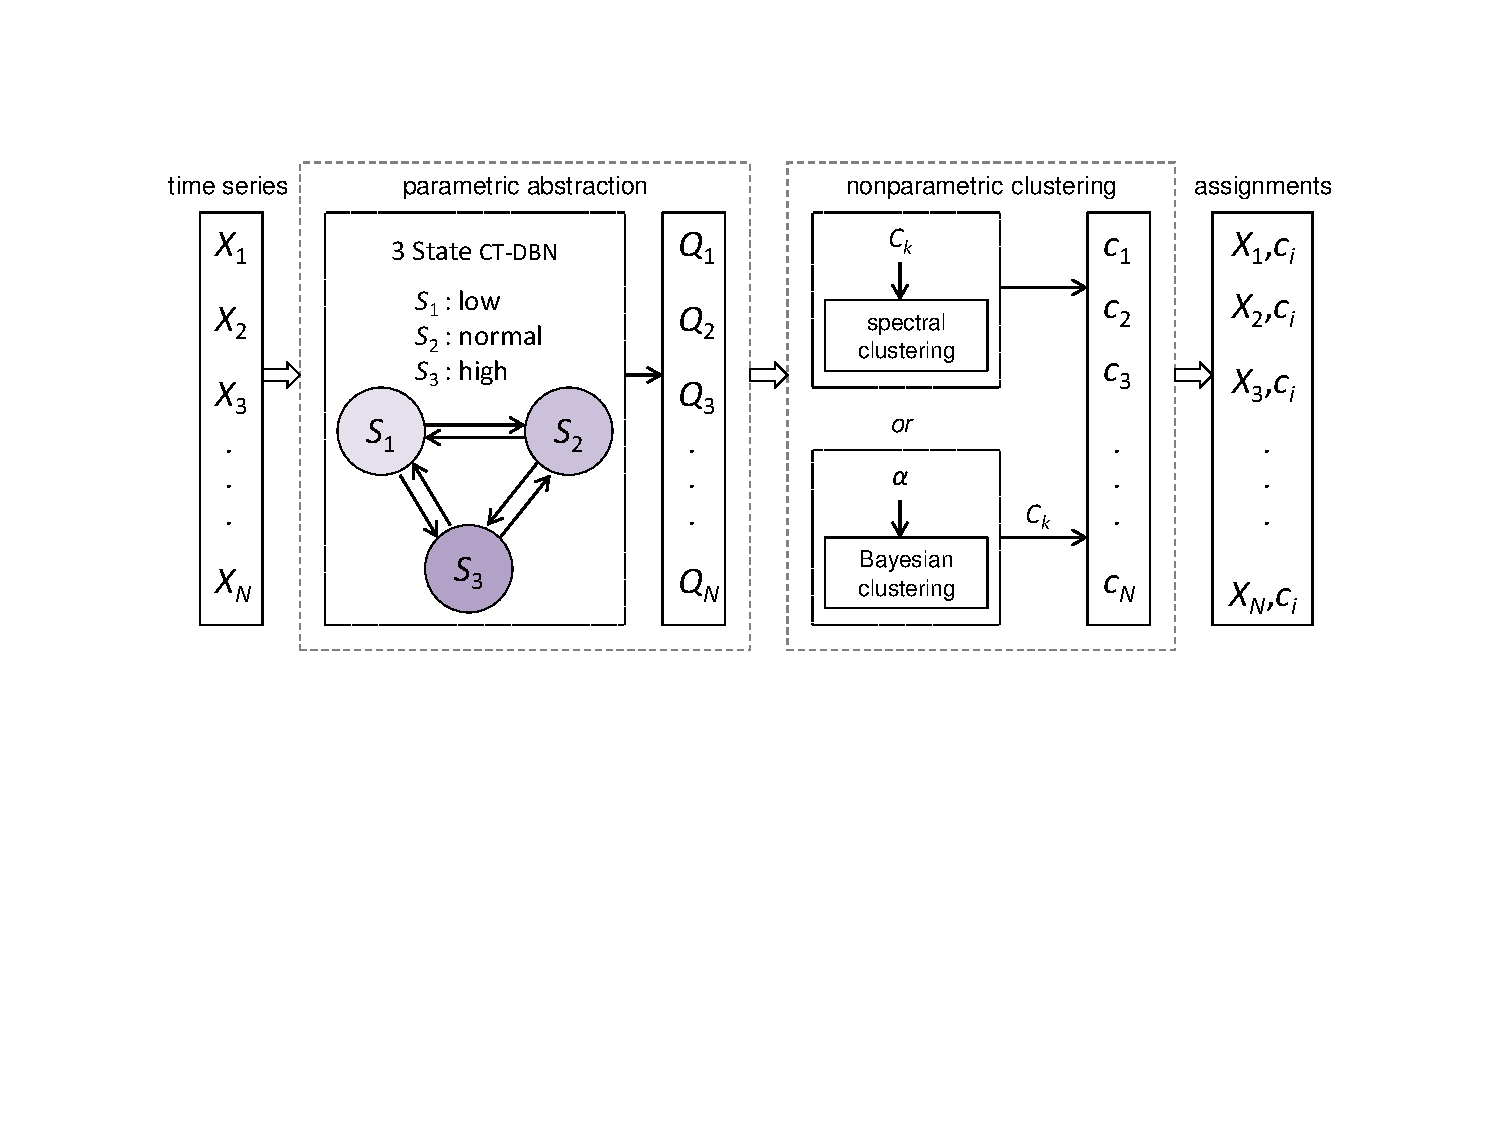
\includegraphics[width=\columnwidth]{fig/semipoverview.jpg}}
\caption{Semiparametric Clustering}
\label{semipar}
\end{center}
\vskip -0.2in
\end{figure}

%temporal clustering
The first step entails temporal abstraction using a parametric model to transform a set of raw time series, $X_1,X_2,...,X_N$, into a more manageable form for traditional multivariate clustering algorithms. It entails learning each patients model-specific parameters, $Q_1,Q_2,...,Q_N$, from the time series observations.  The second step is nonparametric clustering.  Spectral methods are typically used in the semiparametric framework, which requires determining the number of clusters, $k$, in advance.  In this work, we extend the clustering component to the nonparametric Bayesian setting, allowing for the number of clusters to be expressed as a function of the sample size.


\subsection{Continuous and Discrete-time Models}
 By default Markov models and dynamic Bayesian networks (DBNs), of which a hidden Markov model (HMM) is the simplest representation, discretize the time trajectory into uniform length contiguous segments, that are assumed to be approximately Markovian to enable tractable inference.  The smallest temporal granularity among all sequences, $\Delta$, denotes a fixed length interval that is repeated at each time slice, where a the template models is also repeated.

 Although discrete-time models are suitable in many cases, there are two key limitations that have been noted in graphical modeling problems~\cite{Nodelman02} and we describe their relevance to modeling EHR data. First, if the underlying health phenomena progresses in individuals at different rates, one granularity must be used to express time steps for the entire system. Second, when data is unavailable, intervening time slices must still be represented.  When data is sparse, this forces the assumption of many unknown values that are propagated through the discrete time model's transition matrix at each $\Delta t$ without support.

%Various examination schemes are possible in the clinical setting and their impact on longitudinal chronic disease studies have been studied\cite{gruger}.  Fixed, random and examination schemes for severely ill patients under a doctor's care have been shown to be non-informative.  However, \emph{self-selection}, which is often driven by a patient's need to see formal care when they are in a poor condition is informative, indicating the missing at random assumption for longitudinal analysis of chronic disease patients is not realistic.  An EHR that provides a comprehensive view of a patients clinical care, makes it more likely to assume that missing data corresponds with a patient absent of disease related symptoms.  However, the fragmentation of patient data mirrors that of the larger US health care system.  A patient seeking care at another provider is not easily known, and estimating values in the absence can be problematic.  A recent simulation study that modeled patient data with DT-HMMs~\cite{YehCS12} assessed the impact of missing observations for various scenarios, and concluded that there is substantial impact on parameter estimates when the data is not missing completely at random and the missing data mechanism in non-ignorable.

When there are no natural time slices, continuous-time DBNs (CT-DBNs)~\cite{Nodelman02} can be used to more directly reflect sequential dependencies, and avoid discretizing the time intervals.  Notably, the class of probabilistic graphical models known in epidemiology and biostatistics as Multi-state models (MSMs), some of which qualify as CT-DBNs, were developed independently of work in computer science and share their foundation in stochastic process theory.

%For chronic disease modeling, biostaticians have noted that discrete time model are an inappropriate citing arbitrary sampling that must be considered and the time course of progression, which may not be linear and evolves at different rates among patients. CT-DBNs, primarily continuous-time hidden Markov models (HMM) have be used to model health decline for variety of conditions including lung disease, and HIV~\cite{Jackson10}.  Also, CT-HMMs have been applied to discovering disease relationships and to overcome the drawbacks of discrete-time models for predicting disease interactions in mental health, and their effectiveness has been demonstrated on a recent, large-scale study~\cite{Murillo}.

%Notably, the class of probabilistic graphical models known in epidemiology and biostatistics as Multi-state models (MSMs).  Not all MSM models are CT-DBNs.  However, many of their extensions for modeling latent variables and covariances, which can be viewed as specialized instance of CT-DBNs applied for modeling disease dynamics.  Although they were developed independently of work in computer science, they share the same grounding in stochastic process theory and share similarities for representation, learning and inference.  MSM were motivated by the limitations of discrete time stochastic processes for modeling disease dynamics from longitudional data with missing observations, or \emph{panel data}~\cite{Jackson10}.

MSMs have a set of rules that govern their design and interpretation and have be used to model a variety of diseases including cardiac disease, cancer, and HIV~\cite{Jackson10}. In terms of structure, nodes represent disease states that are ordered progressively to reflect stages in a disease trajectory.  A patient with chronic diseases may traverse these nodes as their disease progresses, and typical MSM states correspond with `healthy', `diseased', and `diseased with complications'.  In the case of applications to survival analysis, a final absorbing state that has no outbound transitions is used to indicate death. Also, for modeling latent states, is common for an MSM emission matrix to reflect diagnostic misclassification error, and there are techniques to estimate initial values based on sensitivity and specificity.

